%%%%%%%%%%%%%%%%%%%%%%%%%%%%%%%%%%%%%%%%%%%%%%%
%%%     Declarations (skip to Begin Document, line 88, for parts you fill in)
%%%%%%%%%%%%%%%%%%%%%%%%%%%%%%%%%%%%%%%%%%%%%%%

%%\documentclass[10pt]{article}
%%\documentclass[10pt]{report}
\documentclass[letterpaper]{article}
\usepackage{geometry}
\usepackage{xcolor}
\usepackage{amsmath}
\usepackage[some]{background}
%\usepackage{lipsum}
%\usepackage{natbib}
\usepackage[backend=biber, bibstyle=numeric, citestyle=numeric]{biblatex}  
%\usepackage{biblatex} 
\addbibresource{paperpile.bib}

% Tables
\usepackage{float}
\usepackage[utf8]{inputenc}
\usepackage{tabularx}
\usepackage{booktabs}
\usepackage{longtable}

\usepackage{diagbox} %table split headers
\usepackage{longtable}
\usepackage{array}
\usepackage{rotating}
\usepackage{eqparbox}
\usepackage{makecell, caption, booktabs}

%

\usepackage{geometry}  % Lots of layout options.  See http://en.wikibooks.org/wiki/LaTeX/Page_Layout
\geometry{letterpaper}  % ... or a4paper or a5paper or ... 
\usepackage{fullpage}  % somewhat standardized smaller margins (around an inch)
\usepackage{setspace}  % control line spacing in latex documents
\usepackage[parfill]{parskip}  % Activate to begin paragraphs with an empty line rather than an indent

\usepackage{amsmath,amssymb}  % latex math
\usepackage{empheq} % http://www.ctan.org/pkg/empheq
\usepackage{bm,upgreek}  % allows you to write bold greek letters (upper & lower case)

% for typsetting algorithm pseudocode see http://en.wikibooks.org/wiki/LaTeX/Algorithms_and_Pseudocode
\usepackage{algorithmic,algorithm}  

\usepackage{graphicx}  % inclusion of graphics; see: http://en.wikibooks.org/wiki/LaTeX/Importing_Graphics
% allow easy inclusion of .tif, .png graphics
\DeclareGraphicsRule{.tif}{png}{.png}{`convert #1 `dirname #1`/`basename #1 .tif`.png}

% \usepackage{subfigure}  % allows subfigures in figure
\usepackage{caption}
\usepackage{subcaption}

\usepackage{xspace}
\newcommand{\latex}{\LaTeX\xspace}

\usepackage{color}  % http://en.wikibooks.org/wiki/LaTeX/Colors

\long\def\todo#1{{\color{red}{\bf TODO: #1}}}

\long\def\ans#1{{\color{blue}{\em #1}}}
\long\def\ansnem#1{{\color{blue}#1}}
\long\def\boldred#1{{\color{red}{\bf #1}}}
\long\def\boldred#1{\textcolor{red}{\bf #1}}
\long\def\boldblue#1{\textcolor{blue}{\bf #1}}

% Useful package for syntax highlighting of specific code (such as python) -- see below
\usepackage{listings}  % http://en.wikibooks.org/wiki/LaTeX/Packages/Listings
\usepackage{textcomp}

% bem: insertions
\usepackage{listings}

%%% The following lines set up using the listings package
\renewcommand{\lstlistlistingname}{Code Listings}
\renewcommand{\lstlistingname}{Code Listing}

%%% Specific for python listings
\definecolor{gray}{gray}{0.5}
\definecolor{green}{rgb}{0,0.5,0}

\lstnewenvironment{python}[1][]{
\lstset{
language=python,
basicstyle=\footnotesize,  % could also use this -- a little larger \ttfamily\small\setstretch{1},
stringstyle=\color{red},
showstringspaces=false,
alsoletter={1234567890},
otherkeywords={\ , \}, \{},
keywordstyle=\color{blue},
emph={access,and,break,class,continue,def,del,elif ,else,%
except,exec,finally,for,from,global,if,import,in,i s,%
lambda,not,or,pass,print,raise,return,try,while},
emphstyle=\color{black}\bfseries,
emph={[2]True, False, None, self},
emphstyle=[2]\color{green},
emph={[3]from, import, as},
emphstyle=[3]\color{blue},
upquote=true,
morecomment=[s]{"""}{"""},
commentstyle=\color{gray}\slshape,
emph={[4]1, 2, 3, 4, 5, 6, 7, 8, 9, 0},
emphstyle=[4]\color{blue},
literate=*{:}{{\textcolor{blue}:}}{1}%
{=}{{\textcolor{blue}=}}{1}%
{-}{{\textcolor{blue}-}}{1}%
{+}{{\textcolor{blue}+}}{1}%
{*}{{\textcolor{blue}*}}{1}%
{!}{{\textcolor{blue}!}}{1}%
{(}{{\textcolor{blue}(}}{1}%
{)}{{\textcolor{blue})}}{1}%
{[}{{\textcolor{blue}[}}{1}%
{]}{{\textcolor{blue}]}}{1}%
{<}{{\textcolor{blue}<}}{1}%
{>}{{\textcolor{blue}>}}{1},%
%framexleftmargin=1mm, framextopmargin=1mm, frame=shadowbox, rulesepcolor=\color{blue},#1
framexleftmargin=1mm, framextopmargin=1mm, frame=single,#1
}}{}
%%% End python code listing definitions

\DeclareMathOperator{\diag}{diag}
\DeclareMathOperator{\cov}{cov}


%\bibliography{./paperpile.bib}
\author{Evan McGinnis}
\title{Parameter Selection for Weed/Crop Discrimination}



\definecolor{titlepagecolor}{cmyk}{1,.60,0,.40}

\DeclareFixedFont{\bigsf}{T1}{phv}{b}{n}{1.5cm}

\backgroundsetup{
scale=1,
angle=0,
opacity=1,
contents={\begin{tikzpicture}[remember picture,overlay]
 \path [fill=titlepagecolor] (-0.5\paperwidth,5) rectangle (0.5\paperwidth,10);  
\end{tikzpicture}}
}
\makeatletter                       
\def\printauthor{%                  
    {\large \@author}}              
\makeatother
\author{%
    Evan McGinnis \\
    Graduate Student, Biosystems Engineering Dept \\
    INFO 529
    \texttt{evanmc@email.arizona.edu}\vspace{40pt} \\
    }
\begin{document}
\begin{titlepage}
\BgThispage
\newgeometry{left=1cm,right=4cm}
\vspace*{1cm}
\noindent
%%\vspace*{0.4\textheight}
\textcolor{white}{\Huge\textbf{\textsf{Parameter Selection in\\ Weed/Crop Discrimination}}}
\vspace*{2.5cm}\par
\noindent
\begin{minipage}{0.35\linewidth}
    \begin{flushright}
        \printauthor
    \end{flushright}
\end{minipage} \hspace{15pt}
%
\begin{minipage}{0.02\linewidth}
    \rule{1pt}{175pt}
\end{minipage} \hspace{-10pt}
%
\begin{minipage}{0.6\linewidth}
\vspace{5pt}
    \begin{abstract} 
This paper is an analysis of various parameters extracted from vegetation images. These parameters are used in KNN, Logistic Regression, Random Forest, and Support Vector Machine to discriminate between crop (cultivars of lettuce) and weeds.
    \end{abstract}
\end{minipage}
\end{titlepage}
\restoregeometry
\tableofcontents
\listoffigures
\newpage
%
% I N T R O D U C T I O N
%
\section{Introduction}
This paper is part of a larger effort to detect weeds in imagery gathered under field conditions and treat those weeds in real-time. More precisely, weed detection with an image must be complete with 100s of milliseconds to treat weeds at commercially viable speeds. While such concerns are beyond the scope of this paper, we will instead focus on selecting object parameters that result in the most accurate predictions of the classification of vegetation into one of two categories: weed or crop. It is of no concern what specific species of weed or crop cultivar -- all that is important here is a binary classification of weed or not weed.\\
The dataset examined in this paper was gathered in an agricultural reasearch field in Yuma, Arizona by capturing images while walking beside a planting bed. The processing of this image set follows this procedure:
\begin{enumerate}
	\item{Segment images (remove pixels that are not vegetation)}
	\item{Label vegetation as weed or crop}
	\item{Extract various parameters from  vegetation images}
	\item{Evaluate signficance of parameters to assigned class}
	\item{Evaluate predictions with various models using selected parameters}
\end{enumerate}

%
% I M A G E  S E G M E N T A T I O N
%
\section{Image Segmentation}
The portions of the images that did not contain pixels with vegetation present were discarded. These images were segmented using various visible light indices \cite{Wirth2004-li}. As this process is not the primary subject of this paper, it will be given only superficial mention here.  Various approaches to image segmentation are  summarized in Table \ref{fig:indices}.

%
% T A B L E  O F  S E G M E N T A T I O N  F O R M U L A E
%
% A bit more space on the table rows, so everything does not look so cramped
{\renewcommand{\arraystretch}{2}%
\begin{table}[H]
%\begin{longtable}{ccc}
    \caption{Visible light indices (\cite{Hamuda2016-dw,Hunt2013-ih})}
    \label{fig:indices}
    \begin{tabular}{  l  p{4cm}  p{5cm} }
        \toprule
\textbf{Index}      
& \textbf{Formula}   
& \textbf{Comment} \\\midrule
Triangular Greeness
& \begin{minipage}[t]{0.3\textwidth}
	$R_{green} - \alpha R_{red} - \beta R_{blue}\\ \alpha = \frac {2(\lambda_{blue} - \lambda_{green})} {(\lambda_{blue} - \lambda_{red})}\\ 
    	\beta = \frac {2(\lambda_{green} - \lambda_{red})} {(\lambda_{blue} - \lambda_{red})} $
   \end{minipage}     
& Corrects for camera calibration using the peak sensitivity \\\hline
Normalized Difference     
& $128 * \left( \left( \frac {(G - R)} {(G + R)} \right) + 1 \right) $                    
& The NDI index produces a near-binary image.  \\\hline
Excess Green      
& \begin{minipage}[t]{0.3\textwidth}
	$R = \frac {R} {R_{max}}\\ G = \frac {G} {G_{max}}\\ B = \frac {B} {B_{max}}$ 
   \end{minipage}
& ExG provided a clear contrast between plants and soil \\\hline
Excess Red      
& $1.3 R - G$ 
& inspired by the fact that there are 4\% blue, and 32\% green, compared with 64\% red cones in the retina of the human eye \\\hline
Color Index of Vegetation Extraction      
& $0.441 R - 0.811 G + 0.385 B + 18.78745$
& This method was proposed to separate green plants from soil background in order to evaluate the crop growing status. \\\hline
Excess Green - Excess Red   
& $ExG - ExR$ 
& ExG used to extract the plant region and ExR used to eliminate the background noise (soil and residue) where green–red material (stems, branches, or petioles) may exist \\\hline
Normalized Green-Red Difference    
& $\frac {(G - R)} {(G + R)}$ 
& The method of NGRDI was used to overcome the differences in exposure settings selected by the digital camera when acquiring aerial photography of the field. \\\hline
Vegetative Index      
& $\frac {G} {R^aB^{(1-a)}}, a = 0.667$ 
& VEG has a significant advantage because it is robust to lighting change.\\\hline
Com1   
& $ExG + CIVE + ExGR + VEG$ 
& TODO \\\hline
Modified Excess Green      
& $1.262G - 0.884R = 0.311B$ 
& TODO \\\hline
Combined Indices 2      
& $0.36ExG + 0.47CIVE + 0.17VEG$ 
& Uses weighting factors to emphasize strengths of various approaches\\\hline    

        \bottomrule
    \end{tabular}
\end{table}
%\end{longtable}
These indices are used to create a mask that is then applied to the original source image to permit vegetation to show while masking details that are not relevant (ground pixels, stones, and other items that may appear in field conditions) The intent here is to remove all pixels that are not relavent to the task of distinguishing between crop and weed:\footnote{Observers will note that the segmentation photo is rotated. This bears further investigation, but will have no impact on the features examined here.}
\begin{figure}[H]
\centering
\begin{subfigure}[]{.32\textwidth}
  \centering
  \includegraphics[width=1\linewidth]{figures/before-segmentation.jpg}
  \caption{Field view of lettuce and weed}
  \label{fig:sub1}
\end{subfigure}
\begin{subfigure}{.32\textwidth}
  \centering
  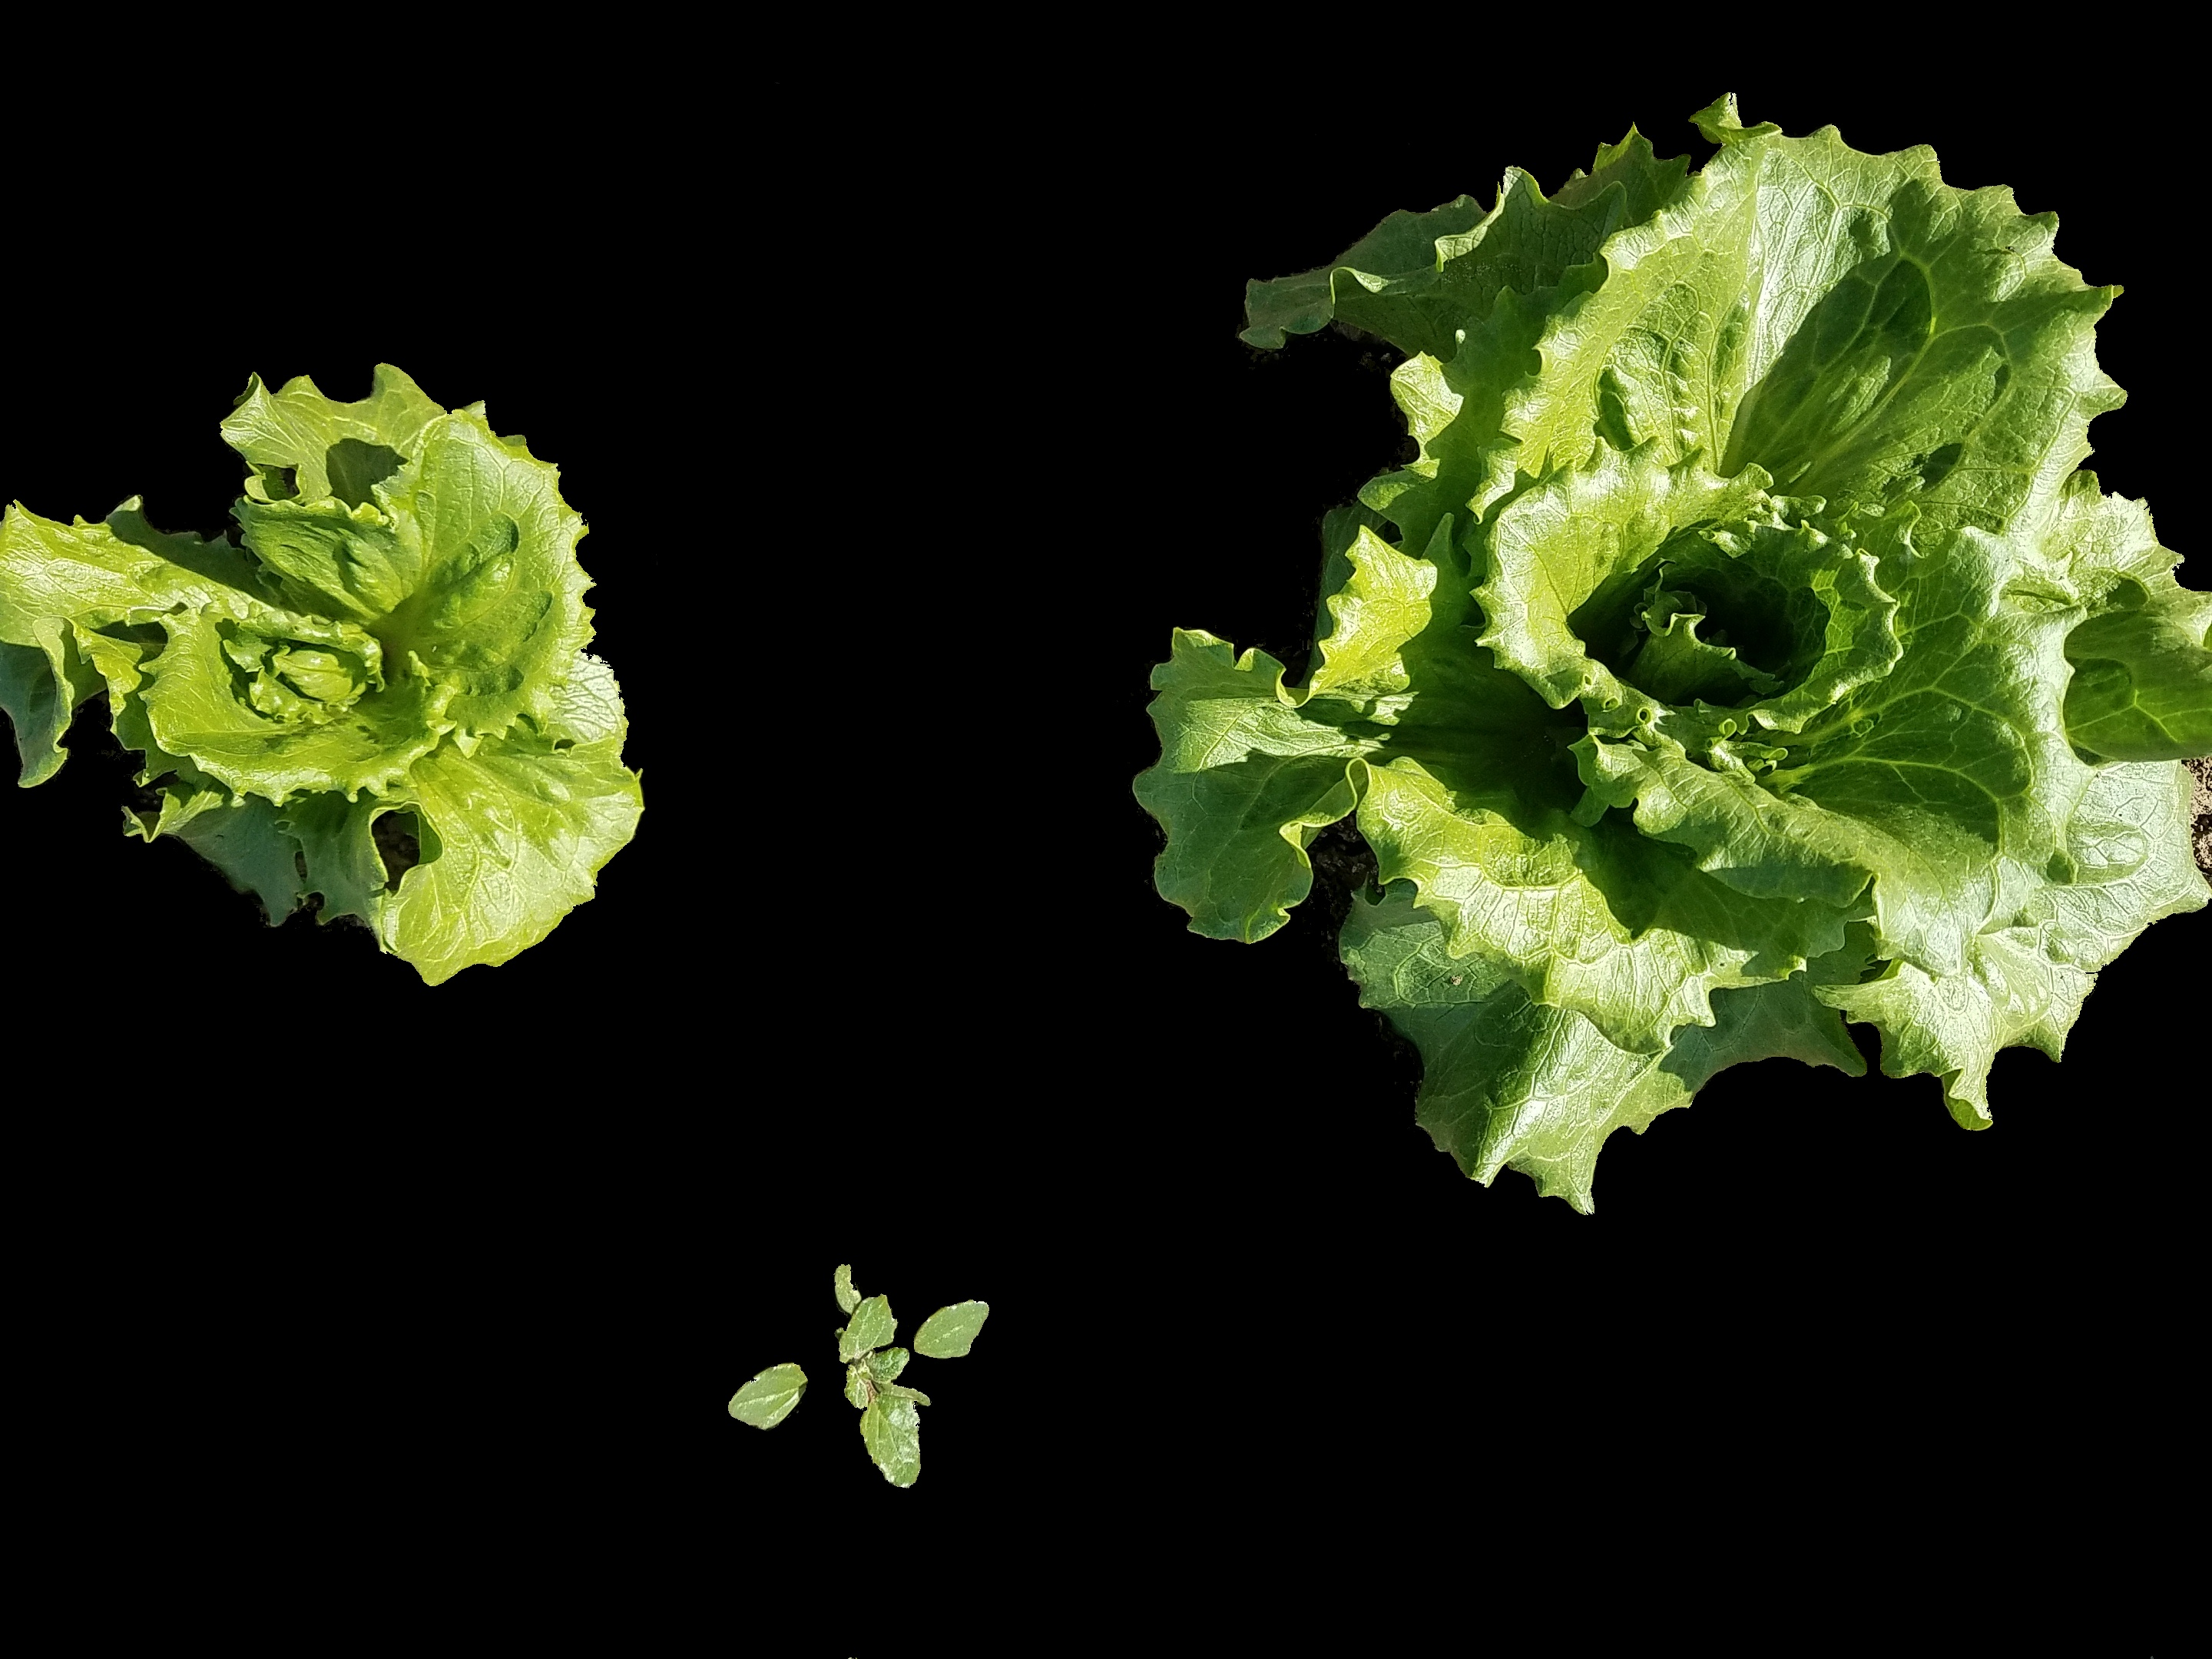
\includegraphics[width=1\linewidth]{figures/after-segmentation.jpg}
  \caption{After segmentation using NDI}
  \label{fig:sub2}
\end{subfigure}
\caption{Before and after segmentation}
\label{fig:segmentation}
\end{figure}
The segmented image has discarded ground pixels while retaining most of the pixels that will be used, but a close examination reveals that pixels in the stems of the weed are also eliminated, as they are less green than the rest of the plant. While they are not eliminated, pixels in the area of the deep shadows of the vegetation may affect attempts to classify objects based on color attributes. It is also envisioned that in the field images will be aquired under controlled, not ambient lighting conditions. For the purposes of this paper, images will use the NDI segmentation approach.


\section{Feature Extraction}
The library used for feature extraction is the OpenCV toolkit, so the discussion of various features may inadvertently slip into using OpenCV terms. Some basic shape descriptors are used below, and the most fundamental ones that apply here are the bounding box, the rectangular box that completely encloses the object, and the convex hull (and convex area), the smallest set of straight lines that completely contains an object. The concept of a {\it centroid} is also important to this discussion.  A centroid is the center of mass of an object, and a concept that will be used in this analysis.

The segmented images produced are then processed by a first identifying the separate objects (often called blobs) within the image and then computing various aspects of each of those objects. Weeds or crop may tend to exhibit these features to an extent that they can be used to distinquish between the two.  Weeds, for instance, may be more elongated than crop, or may tend to have saturation differences that may not be readily apparent to the casual observer.
\subsection{Length Width Ratio}
The ratio of width to length is not -- as the name might imply -- a simple ratio, but is expressed as:
\begin{eqnarray*}
S = 
	\begin{bmatrix}
	Var(X) & Cov(XY) \\[0.3em]
	Cov(XY) & Var(Y) \\[0.3em]
	\end{bmatrix},
\lambda = \frac {eig_{1}(S)} {eig_{2}(S)}
\end{eqnarray*}
Where $eig_{1}(S)$ and $eig_{2}(S)$ are the maximum eigenvalues of the matrix $S$, with $\lambda$ representing the ratio. \cite{Lin2017-xq}
\subsection{Shape Index}
The shape index of an object is a metric expressing the relationship between an object's perimeter and its area.
\begin{eqnarray*}
\alpha = \frac {e} {4 \sqrt{A}}
\end{eqnarray*}

\subsection{Normalized Distance from Cropline}
The cropline in a planting is, simply, the line along the bed where crop can be expected. Under field conditions the cropline will appear in the same spot in each photo. The image set here, however, was manually acquired by walking along the crop row and capturing images.  Unfortunately, this means that the crop line location will differ from one picture to another. For this image set, the cropline is defined as the line that intersects the centroid of the objects with the largest area. Crops will most often have a distance from the cropline very close to zero. Weeds, on the other hand, may have a distance close to zero if they appear within the line of crop, but often appear far from the crop line.
\begin{figure}[h!]
	\centering
	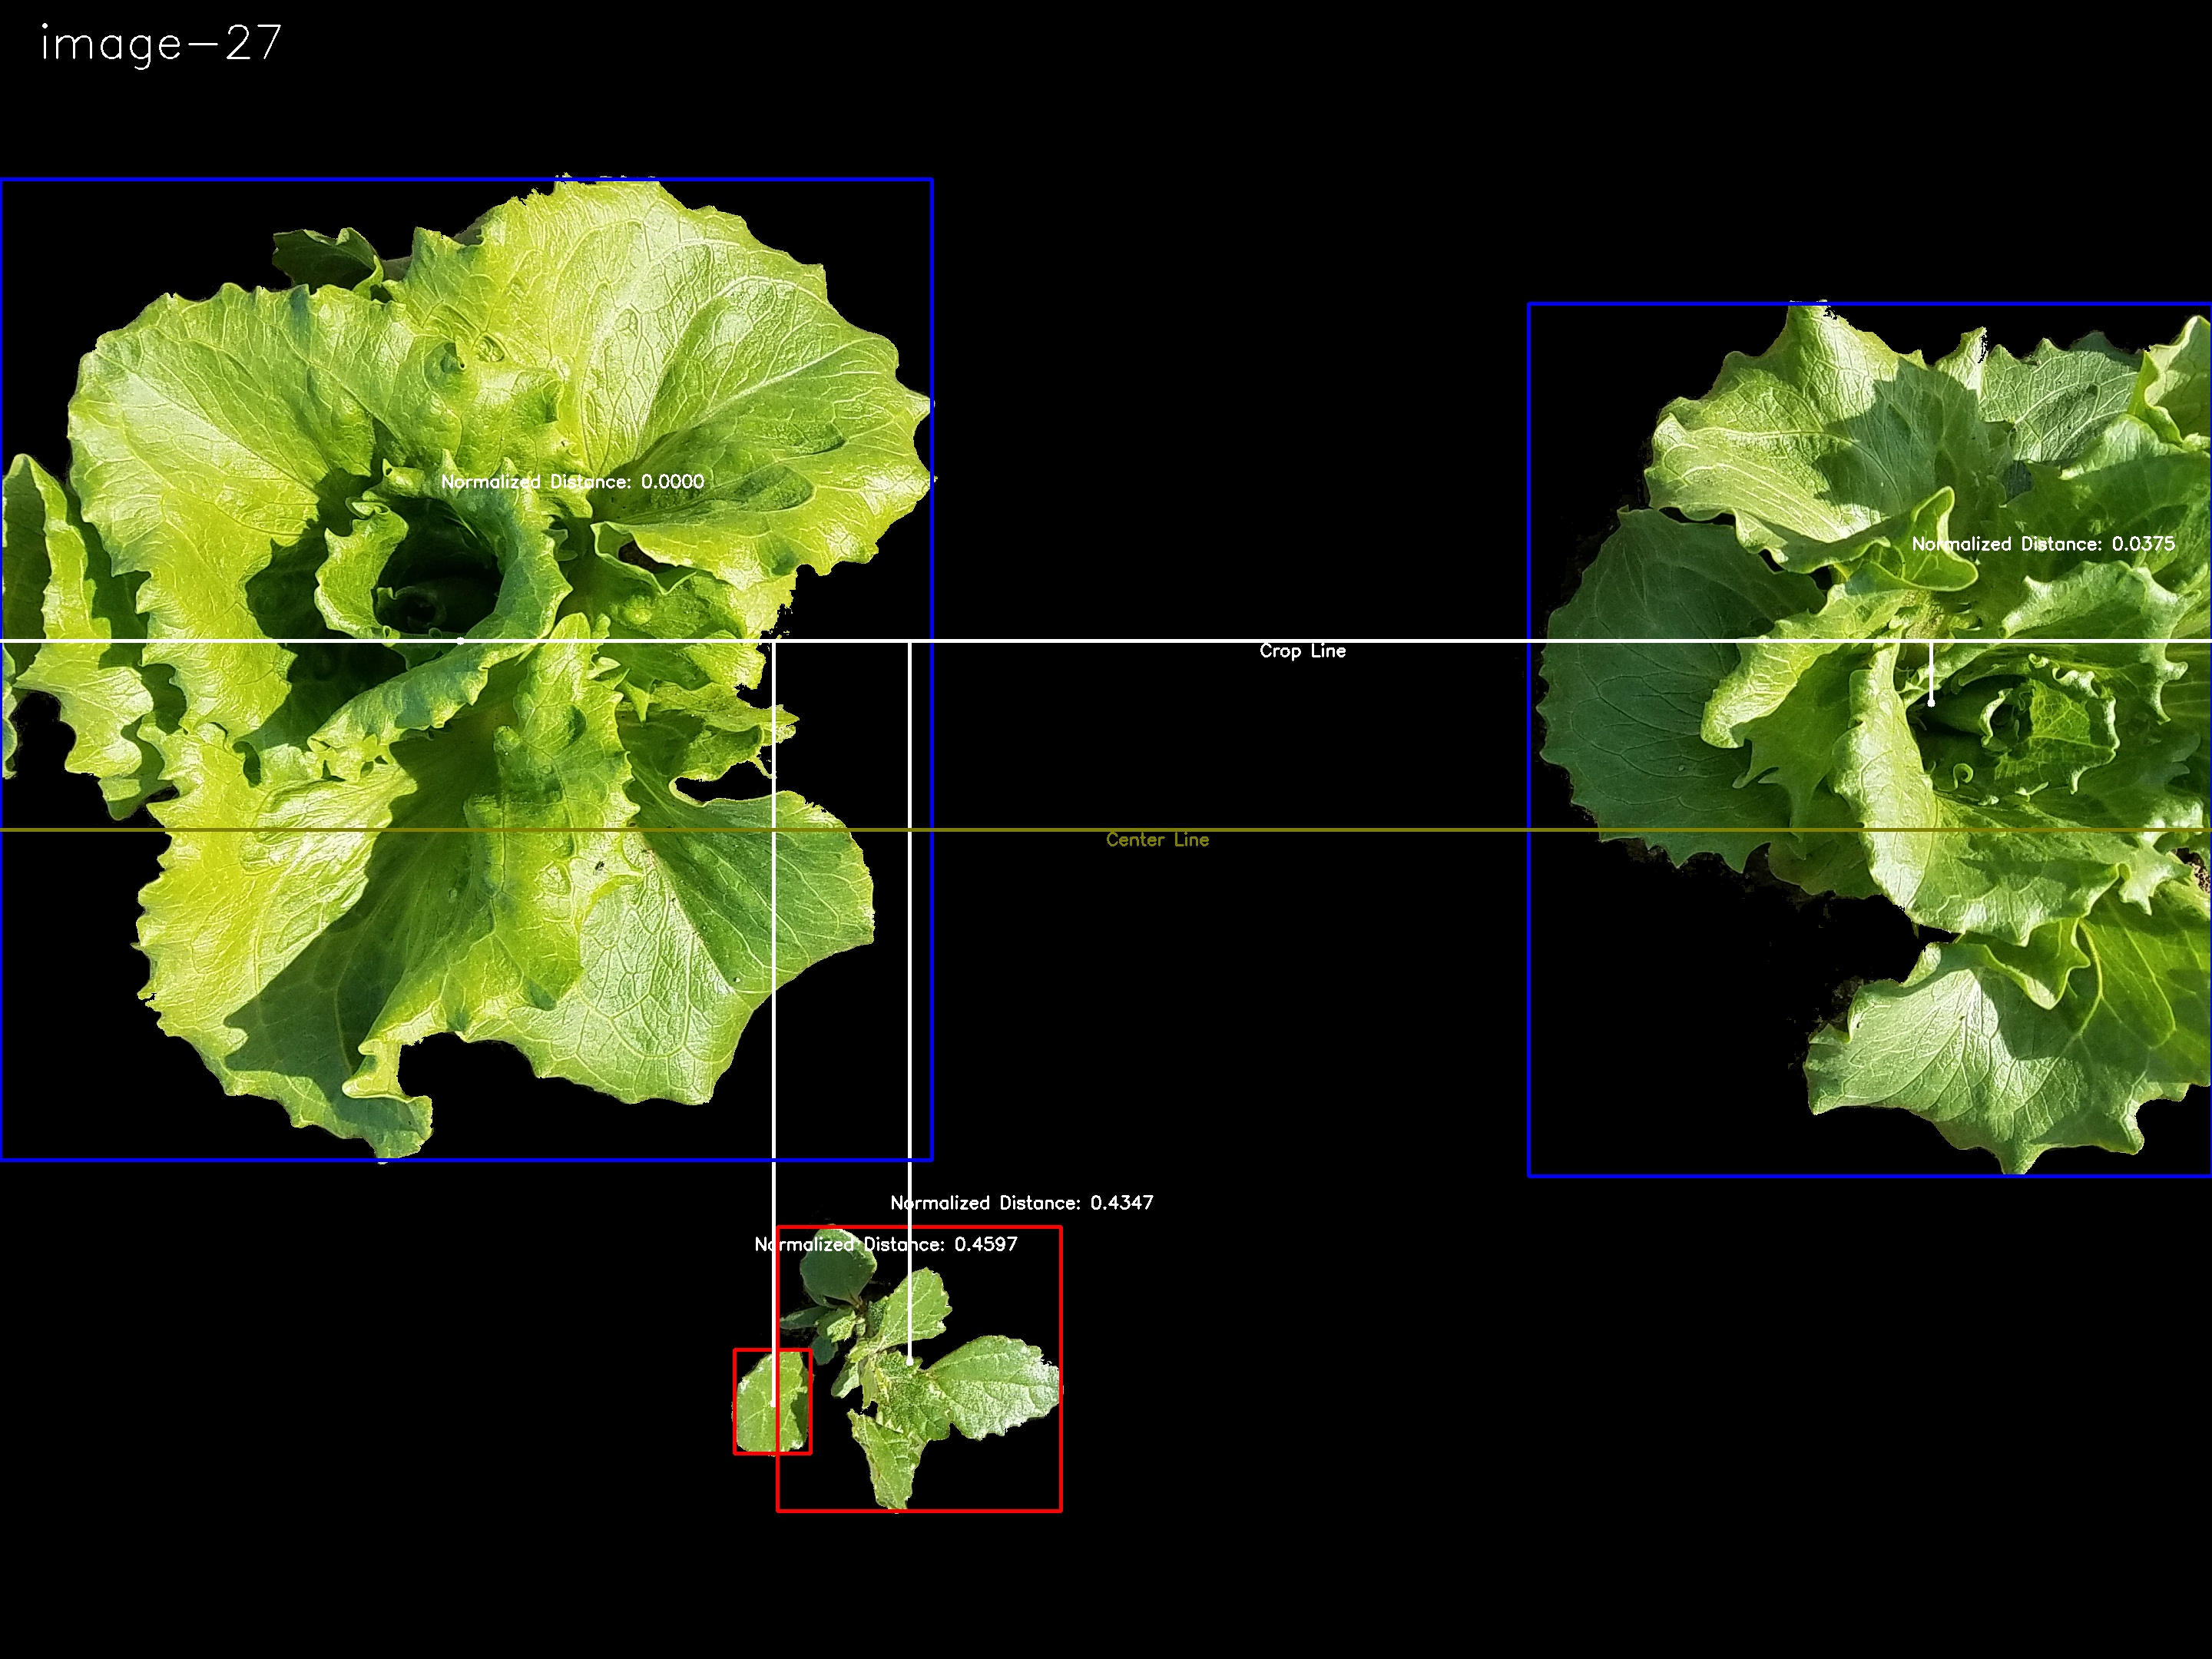
\includegraphics[width=0.4\linewidth]{./figures/normalized-distance.jpg}
	\caption{Normalized Distance to Cropline (Source: author)}
	\label{fig:normalized-distance}
\end{figure}
Figure~\ref{fig:normalized-distance} illustrates the concept of a cropline and the normalized distance of vegetation from it. In this image we see two growths of lettuce that are very close to the cropline (distances here are in pixels, but the units are not significant. This could be expressed in millimeters) at 0 and 0.375 and a weed lying 0.4347 units from the cropline. The line marked {\it Center Line} is for reference purposes and can be ignored for now.  There are two additional items that are worth noting about this image: the dots connecting the plant to the cropline are the {\it centroids} mentioned earlier, and the colored bounding boxes signify the class of the object, something we will return to in a later section.

\subsection{Hue}
The hue of an object is define TODO: Insert an actual definition. In this case, the image is converted to the Hue Saturation and Intensity colorspace and the mean value for the hue is taken.
\subsection{Saturation}
In this case, the image is converted to the Hue Saturation and Intensity colorspace and the mean value for the saturation is taken.
\subsection{YIQ}
The YIQ model of color us used by the NTSC color TV system. Y represents the luma information, I and Q the chrominance information. The processing employed here is to convert the image to the YIQ color space and take the mean value for the I, or in-phase component.
\begin{figure}[h!]
	\centering
	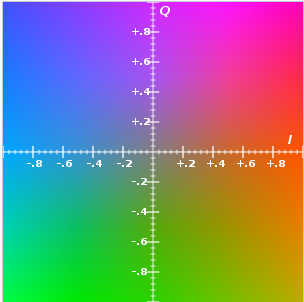
\includegraphics[width=0.4\linewidth]{./figures/yiq.png}
	\caption{YIQ (Source: \cite{Various_undated-cz})}
	\label{fig:yiq}
\end{figure}
The $I$ component is the feature of interest here, and conversion of RGB to YIQ is achieved with this transformation:
\begin{eqnarray*}
	\begin{bmatrix}
	Y \\[0.3em]
	I \\[0.3em]
	Q \\[0.3em]
	\end{bmatrix}
	\approx
	\begin{bmatrix}
	0.299 & 0.587 & 0.114 \\[0.3em]
	0.5959 & -0.2746 & -0.3213\\[0.3em]
	0.2115 & -0.5227 & 0.3112 \\[0.3em]
	\end{bmatrix}
	\begin{bmatrix}
	R \\[0.3em]
	G \\[0.3em]
	B \\[0.3em]
	\end{bmatrix}	
\end{eqnarray*}

\subsection{Compactness}
The compactness of an object is defined as the ratio of its area to the area of a circle with the same perimeter as the original object, and is given by this equation \cite{Wirth2004-li}:
\begin{eqnarray*}
\frac {4 \pi\ area} {perimeter^2}
\end{eqnarray*} 
The most compact object is a circle, whose value is computed as $1$.  Objects with irregular boundaries will have values larger than 1.
\begin{figure}[H]
	\centering
	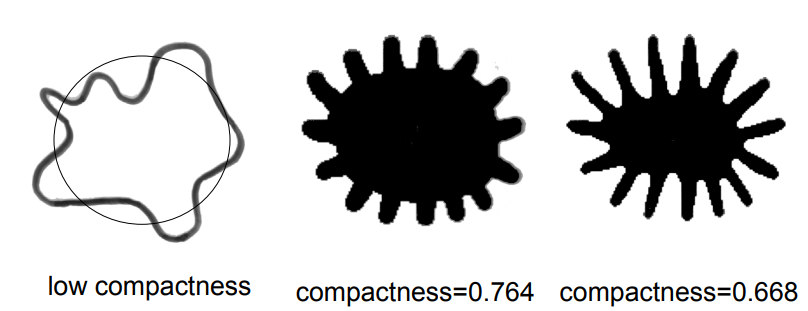
\includegraphics[width=0.4\linewidth]{./figures/compactness.png}
	\caption{Examples of compactness Source:~\cite{Wirth2004-l}}
	\label{fig:compactness}
\end{figure}

\subsection{Elongation}
Elongation is the ratio of the length to the width of an object's bounding box \cite{Wirth2004-li}:
\begin{eqnarray*}
\frac {width_{bounding}} {length_{bounding}}
\end{eqnarray*}
This produces a metric between 0 (more elongated) and 1 (roughly circular or square).
\begin{figure}[H]
	\centering
	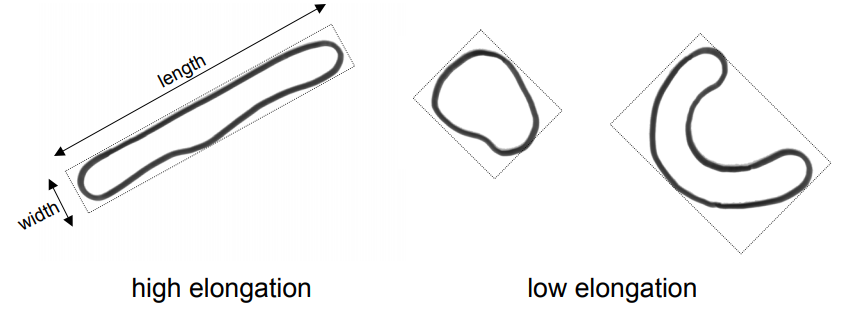
\includegraphics[width=0.4\linewidth]{./figures/elongation.png}
	\caption{Examples of elongation Source: \cite{Wirth2004-l} }
	\label{fig:elongation}
\end{figure}
\subsection{Eccentricity}
The eccentricity (or ellipticity) of an object is the ratio of the length of the minor axis to the length of the major axis. 
\begin{eqnarray*}
\frac {length_{minor-axis}} {length_{major-axis}}
\end{eqnarray*}
The major axis of an object is expressed as the (x,y) endpoints of the longest line that can be drawn through an object. The minor exis is the longest line that can be drawn through an object while remaining perpendicular to the major axis. \cite{Wirth2004-li}
\begin{figure}[H]
	\centering
	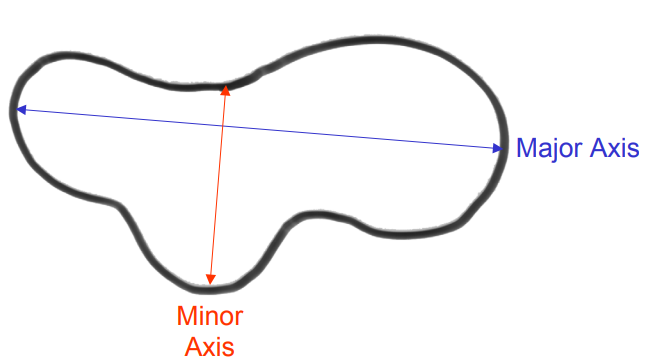
\includegraphics[width=0.4\linewidth]{./figures/major-minor-axis.png}
	\caption{Illustration of major and minor axis Source: \cite{Wirth2004-l} }
	\label{fig:major-minor}
\end{figure}

\subsection{Roundness}
The roundness of an object is an expression varying between 1 (perfectly circular) and 0 (departure from circularity).
\begin{eqnarray*}
\frac {4 \pi\ area} {(convex\ perimeter)^2}
\end{eqnarray*}


\subsection{Convexity}
The convexity of an object is the amount an object differs from a convex object, expressed as the ratio of an object's convex perimeter to the perimeter \cite{Wirth2004-li}:
\begin{eqnarray*}
\frac {convex\ perimeter} {perimeter}
\end{eqnarray*}
\begin{figure}[H]
	\centering
	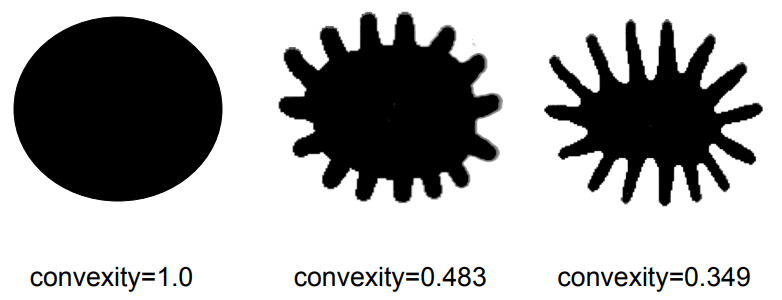
\includegraphics[width=0.4\linewidth]{./figures/convexity.png}
	\caption{Illustration of convexity Source: \cite{Wirth2004-l} }
	\label{fig:circularity}
\end{figure}

\subsection{Solidity}
The solidity of an object varies between 1 (completely solid) and 0, an indication that the object has irregular boundaries.
\begin{eqnarray*}
\frac {area} {convex\ area}
\end{eqnarray*}
\begin{figure}[H]
	\centering
	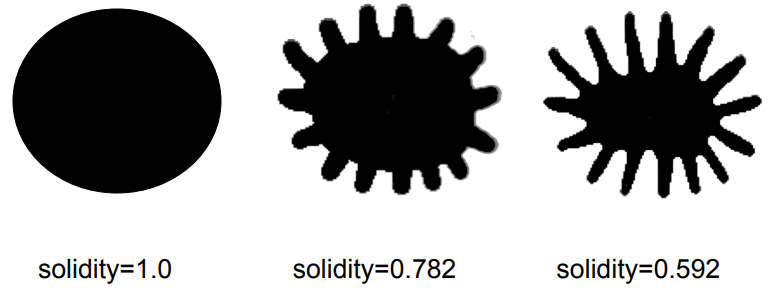
\includegraphics[width=0.4\linewidth]{./figures/solidity.png}
	\caption{Illustration of solidity Source: \cite{Wirth2004-l} }
	\label{fig:circularity}
\end{figure}

\section{Feature Selection}
The features described in the previous section were generated for a set of segmented images, resulting in each object being described by these attributes. Several technique were then used to explore the relationship between these attributes and the labeled class. Specifically, only the most important variables will be selected in the predictions, and those parameters with a weak association will be dropped.
\subsection{Univariate}
In the univariate scheme, the features with the strongest association with the class are selected. In this scheme, scikit-learn supports a suite of statistical tests, and we will use the ANOVA F-value method for feature evaluation.
\subsection{Low Variance}
\subsection{Feature Importance}
The Feature Importance scheme uses Random Forest and Extra Trees approaches to rank features for importance.

Applying this to the dataset created results in these scores, where more important features are assigned higher scores. Table~\ref{fig:importance} shows the results of the scores assigned to the various features.   In this table, we can see that the {\it YIQ}, the {\it Normalized Distance}, and the {\it Compactness} are the most important features. Interestingly, color features play prominently here, far exceeding the scores assigned to structural features such as the {\it Solidity} of an object. Structural features such as {\it Eccentricity} have scores low enough that it is likely the case that they could be omitted from the model without a negative impact on accuracy.

{
\centering\settowidth\rotheadsize{\bfseries(our proposal)}
\renewcommand\theadalign{cl}\renewcommand\cellalign{cl}
\renewcommand\theadfont{\bfseries}
\renewcommand\tabcolsep{4pt}\renewcommand\arraystretch{1.25}
% Make this a bit smaller so it will fit on a page.  Still looks a bit nasty in that it extends to the edge of the page.
% It's that PCA line that is the trouble, as the values are just too long
\footnotesize
\begin{longtable}[c]{
    |l |*{12}{c |} }%
    \hline
    %\diagbox[height=1.2\rotheadsize, width=\dimexpr\eqboxwidth{AB}+2\tabcolsep\relax]%
    %{\raisebox{1.2ex}{Feature}}{\raisebox{-5ex}{Feature}} &
    {\textbf{Feature}} & {\textbf{Importance}}\\
    %\rothead{Tool X\\\mbox{(our proposal)}}\\
    \hline
    \eqmakebox{Length-Width Ratio} & 0.02998853 \\
    \eqmakebox{Shape Index} & 0.05357191 \\
    \eqmakebox{Distance} &  0.05081641 \\
    \eqmakebox{Normalized Distance} & 0.12969820 \\
    \eqmakebox{Hue} & 0.00542753  \\
    \eqmakebox{Saturation} & 0.08911404  \\
    \eqmakebox{YIQ Mean} & 0.38947503  \\
    \eqmakebox{Compactness} & 0.09122537  \\
    \eqmakebox{Eccentricity} & 0.00761004 \\
    \eqmakebox{Roundness} & 0.04467927  \\
    \eqmakebox{Convexity} & 0.05499904   \\
    \eqmakebox{Solidity} & 0.05339462  \\
    \hline
    \caption{Feature Importance Scores}
    \label{fig:importance}
  \end{longtable}
 }
 
 
\subsection{Recursive Elimination}
The Recursive Feature Elimination scheme works backwards from a full model (all attributes) to remove attributes, build a model, and evaluate the results to characterize a feature's contribution to the prediction.
\subsection{Principal Component Analysis}
Principal Component Analysis (PCA) involves re-projecting the data (a change in basis) as a technique to reduce the dimensionality of the data \cite{Muller2016-ui}
\subsection{Feature Importance}


% TODO: Put an example image here


% Put the table in its own object
{
\centering\settowidth\rotheadsize{\bfseries(our proposal)}
\renewcommand\theadalign{cl}\renewcommand\cellalign{cl}
\renewcommand\theadfont{\bfseries}
\renewcommand\tabcolsep{4pt}\renewcommand\arraystretch{1.25}
% Make this a bit smaller so it will fit on a page.  Still looks a bit nasty in that it extends to the edge of the page.
% It's that PCA line that is the trouble, as the values are just too long
\footnotesize
\begin{longtable}{
    |l |*{12}{c |} }%
    \hline
    \diagbox[height=1.2\rotheadsize, width=\dimexpr\eqboxwidth{AB}+2\tabcolsep\relax]%
    {\raisebox{1.2ex}{Selection}}{\raisebox{-5ex}{Feature}} &
    \rotcell{Length-Width Ratio} &
    \rotcell{Shape Index} &
    \rotcell{Distance} &
    \rotcell{Normalized Distance} &
    \rotcell{Hue} &
    \rotcell{Saturation} &
    \rotcell{YIQ Mean} &
    \rotcell{Compactness} &
    \rotcell{Eccentricity} &
    \rotcell{Roundness} &
    \rotcell{Convexity} &
    \rotcell{Solidity}\\
    %\rothead{Tool X\\\mbox{(our proposal)}}\\
    \hline
    \eqmakebox[AB][l]{Univariate} & 23.6 & 120.5 & 70.1 & 138.6 & 1.1 & 134.9 & 517.8 & 115.0 & 0.3 & 38.0 & 1.0 & 34.1 \\
    \eqmakebox[AB]{Variance} & 2.114 & 0.008 & 9150.389 & 0.027 & 117.093 & 1350.474 & $>$0.001 & 0.0376 & 0.174 & 0.174 & 0.312 & 0.014 \\
    % Not sure why these come out centered and the first two are left aligned.
    \eqmakebox[AB]{Recursive} & 3  &2 &12  &1  &9 &10 &11  &4  &7  &5  &8  &6 \\
    %\eqmakebox[LHS]{PCA} & 9.85e-01 & 1.32e-02 & 1.10e-03 & 2.48e-05 & 1.726e-06 & 1.093e-06 & 1.63e-07 & 3.91e-08 & 2.61e-08 & 1.26e-08 & 3.39e-09 & 3.55e-10\\
    \eqmakebox[AB]{Importance} &0.039  &0.070 &0.027 &0.260 &0.033 &0.108 &0.252 &0.087 &0.015 &0.067 &0.011  &0.032\\
    \hline
    \caption{Feature Selection using various approaches.}
    %\label{fig:selection}
  \end{longtable}
 }
  
  
\section{Crop/Weed Discrimination}
\subsection{KNN}
\subsection{Logistic Regression}
\subsection{Support Vector Machine}
\subsection{Random Forest}
\subsection{Boosted Gradient}

\section{Conclusions}
{\renewcommand{\arraystretch}{2}%
\begin{table}[H]
    \caption{Learning Results}
    \label{fig:learning}
    \begin{tabular}{  l  p{4cm}  p{5cm} }
     %\begin{tabular}{  l  p{3.4cm}  p{3.4cm} }
        \toprule
\textbf{Method}      
& \textbf{Train}   
& \textbf{Test} \\\midrule
KNN
& 0       
& 0 \\\hline
Logistic Regression     
& $0$                    
& $0$ \\\hline
SVM      
& $0$ 
& $0$ \\\hline
Random Forest      
& $0$ 
& $0$ \\\hline
    
        \bottomrule
    \end{tabular}
\end{table}
\newpage
\section{References}
\printbibliography[heading=none]

%\cite{Wirth2004-li}
\end{document}

